\chapter{Technische Charakteristiken und Spezifikationen}

\section{Allgemeines Design und technische Voraussetzungen}
Die Hardware besteht aus einem RFID Lesegerätes mit 2 angeschlossenen Antennen. Eine der Beiden Antennen soll sich rund 60cm weiter entfernt befinden und sich direkt neben dem Förderband befinden. Die Zweite Antenne soll sich rund 50cm über dem Förderband befinden und direkt nach unten ausgerichtet sein. Zur Abschirmung zwischen dem Förderband, auf welchem die Tags gemessen werden sollen und dem dahinter befindlichen soll zwischen den beiden Förderbänder eine einfache Aluminium Platte befestigt werden (Siehe \ref{fig:positionAntennen}).

Die Platzierung der Antennen steht in direktem Einfluss mit der Lesbarkeit der Tags, da die Ausrichtung der Tags zur Antenne dazu führen können, dass dieser nicht gelesen werden kann.

\begin{figure}
	\centering
	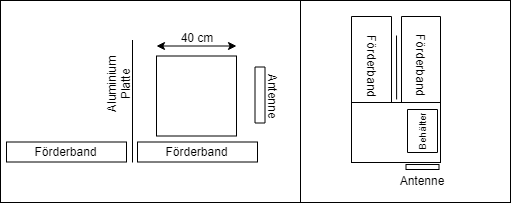
\includegraphics[keepaspectratio,width=\linewidth]{Positionierung_Antennen}
	\caption{Antennenposition eins und zwei}
	\label{fig:positionAntennen}
\end{figure}


Durch die Ausrichtung der Antennen wird weiter vorausgesetzt, dass das Lesegerät mit den Antennen eine maximale Distanz von 53.85cm lesen können. Jeder Behälter enthält gemäss angaben im Normalfall 50 Exemplare, daraus ergibt sich, dass das Lesegerät für den Normalfall mindestens 50 Exemplare in der Zeit auslesen muss, welche das Förderband benötigt um die Kiste ca. 60cm weit zu Transportieren.

\section{Vergleich der vorgeschlagenen Lösung und der existierenden Situation}
Die Existierende Situation enthält momentan noch keine Möglichkeit der Verifikation des Inhaltes eine Behältnisses. Demnach würde durch die Durchführung dieses Projektes die Wahrscheinlichkeit des Deplatzieren massiv verringern.

\section{Gründe für den Vorteil der vorgeschlagenen Lösung}


\section{Vorgeschlagene Zulieferungsquellen und Aquisitionsmethoden}

\section{Geschätzte Kosten und Quellen für die Basis dieser Schätzungen}
